% =====================================================================
% Appendix D -- Drive without speed control, and the validity conditions in full.
% Grip: DIN 22101 sec. 7.3.1 and 8.2.2, Eqs. 47-50.
% Numbers: paper_numbers.py, sections "Validity conditions" and "Take-up kinematics".
% Tests: test_harrison.py::test_damped_drive_limits; test_eigen.py (torque variant
% vs FE); test_validity.py.
% =====================================================================
\section{Drive without speed control and validity conditions}\label{app:driveandvalidity}

\subsection{Drive without speed control}\label{app:torque}\label{sec:torque}

If the drive imposes a torque instead of a velocity, its faces move with an unknown displacement
and the drive acts as a mass $M_d=J_d/R_d^2$ that joins the two ends of the loop ($J_d$ is the
drive inertia reduced to the pulley shaft and $R_d$ the pulley radius). The linearised slip of an
induction motor adds a viscous force towards the reference speed, with coefficient $c_d$. With
$m_d=M_d/(\mu_rL)$ and $\hat c=c_d/(\mu_rc_r)$, the drive conditions become $W(0)=W(2)$ and
$W'(0)-W'(2)=-(m_d\Omega^2-\ii\hat c\,\Omega)\,W(0)$, and the characteristic equation is
\begin{equation}\label{eq:chareq_torque}
  2-\operatorname{tr}\mat P+\left(m_d\Omega^2-\ii\hat c\,\Omega\right)P_{12}=0,
  \qquad \mat P=\mat B\mat J\mat A,
\end{equation}
whose roots are complex when $\hat c>0$ (damped roots have $\operatorname{Im}\Omega>0$). For
$m_d\to\infty$ or $\hat c\to\infty$ it reduces to $P_{12}=0$, the prescribed
velocity~\eqref{eq:chareq}. For $m_d\to0$ and $\hat c=0$ it gives the periodic condition
$\operatorname{tr}\mat P=2$ of a free loop, which has a rigid-body mode: with the take-up next to
the drive, $\beta\to0$ and $\gamma=1$, the fundamental changes from the quarter-wave mode of the
loop under prescribed velocity (period $8L/c_r$) to its half-wave mode (period $4L/c_r$). With
$m_d=0$ and $\beta\to0$ the dashpot alone reflects waves at the drive with the real coefficient
$(\hat c-1)/(\hat c+1)$; for $\hat c>1$ it leaves the period of the prescribed-velocity limit
unchanged and only adds damping, with $\operatorname{Re}\Omega=\pi/[2(2-\xi)]$ and
$\operatorname{Im}\Omega=\ln\bigl[(\hat c+1)/(\hat c-1)\bigr]/[2(2-\xi)]$ for $\gamma=1$ as
$\xi\to0$. The prescribed velocity therefore represents drives whose speed is controlled in
closed loop, as recommended for start-up and stopping of long conveyors \citep{jennings2013} and as
in the frequency-controlled starts of \citet[\S8.6.2]{lodewijks1996}, or whose reduced inertia is
large compared with the mass of the belt. Section~\ref{sec:fieldchecks} and \cref{app:validation} use
Eq.~\eqref{eq:chareq_torque} on Harrison's wound-rotor drive (details in the supplementary
material, S5) and on Lodewijks' conveyor.

\subsection{Validity conditions}\label{app:validity}

\begin{figure}[tbp]
  \centering
  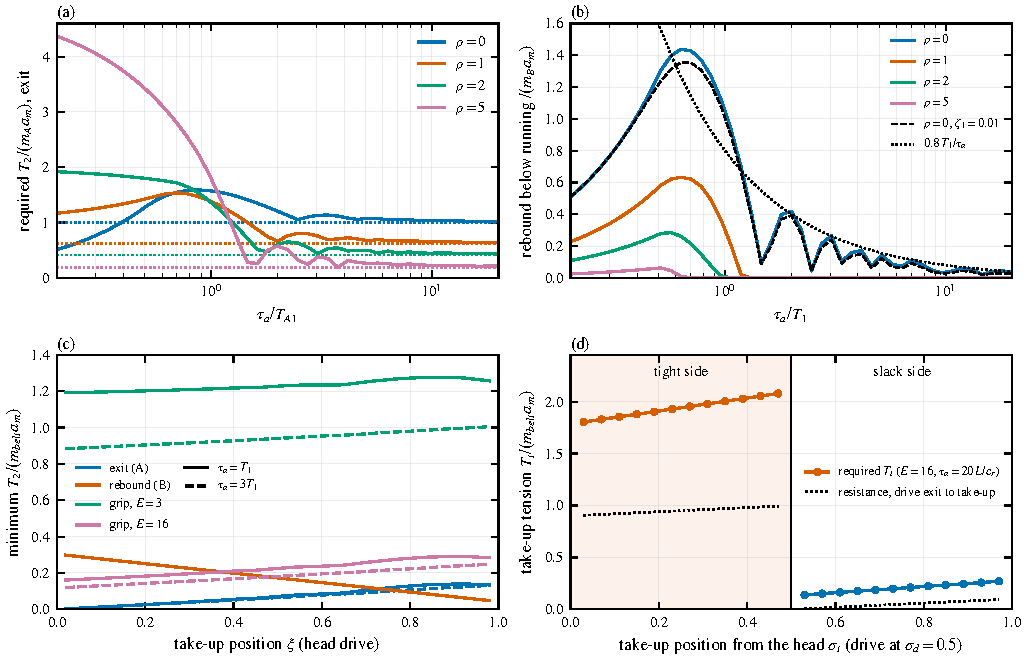
\includegraphics[width=\linewidth]{fig_validity}
  \caption{Validity of the linear model with prescribed drive velocity ($\beta\to0$, sine
  profile, undamped, resistances $r=\rho\,\mu\,a_m$ starting with the belt speed). (a) Running
  tension at the drive exit needed to keep strand~A taut during the start, per unit inertial
  force of strand~A; dotted, the slow-start limit $\sqrt{1+\rho^2/4}-\rho/2$. (b) Rebound of
  strand~B below its running tension after the start: up to \NumReboundMax\,$m_Ba_m$ without
  resistances, zero at $\tau_a=(j+\tfrac12)\,\tauper{1}$ and decaying as about
  $0.8\,\tauper{1}/\tau_a$; dashed, $\zeta_1=0.01$. (c) Minimum running tension $T_2$ against the
  take-up position, head drive, $\gamma=2$, $\rho=1$, for $\tau_a=\tauper{1}$ (solid) and
  $3\tauper{1}$ (dashed): grip governs with a single drive pulley ($\egrip=3$); with a tandem drive
  ($\egrip=16$) slack, rebound and grip are comparable. (d) Take-up tension required with the drive
  at mid-length of the return strand (full loop, $\gamma=2$, $\rho=1$, $\egrip=16$, $\tau_a=20$):
  on the tight side of the drive it is \NumTightMin--\NumTightMax\,$m_\mathrm{belt}a_m$, against
  \NumSlackMin--\NumSlackMax\ on the slack side; dotted, the running resistance between the drive
  exit and the take-up.}
  \label{fig:validity}
\end{figure}

Take resistances proportional to the inertial density, $r=\rho\,\mu\,a_m$ in each strand
($\rho=fg/a_m$ for a common resistance coefficient $f$), starting with the belt speed. The
take-up holds $\Tt=T_2+\rho\,m_Aa_m$, where $T_2$ is the running tension at the drive exit, and
gravity on an inclined path only shifts the static level. Let $C_\mathrm{max}$ and
$C_\mathrm{min}$ be the extremes of the fixed-end tension of a uniform strand under the combined
load, per unit inertial force $m_sa_m$; for $\rho=0$, $C_\mathrm{max}=D$.

\paragraph{(i) Slack} With the take-up as a free end the strands share only $\Tt$, and the belt
can lose tension in two places. During the start the tension at the drive exit drops by the
dynamic tension of strand~A, which requires $T_2\ge m_Aa_m\,[C_\mathrm{max}(t_a/\tper{A1})-\rho]$
(\cref{fig:validity}a). The estimate is exact, since strand~A is uniform; for slow starts it tends
to $m_Aa_m(\sqrt{1+\rho^2/4}-\rho/2)$, and it grows with $\xi$ but remains small: at most
\NumValidityExitMax\,$m_\mathrm{belt}a_m$ for $\gamma=2$, $\rho=1$ and starts of one to three
periods, with $m_\mathrm{belt}=\mu_rL(1+\gamma^2)$. After the start the oscillation left in
strand~B swings the entry tension below its running value, which requires
$T_2\ge-m_Ba_m\,C_\mathrm{min}(t_a/\tper{1})-\rho\,m_Aa_m$ (\cref{fig:validity}b). Without
resistances this rebound reaches \NumReboundMax\,$m_Ba_m$ for fast starts, where after the
reflection at the free end the tension passes from $Z_sV_\infty$ to $-Z_sV_\infty$; it vanishes for
$t_a=(j+\tfrac12)\,\tper{1}$, where the first mode is left at rest, and decays as about
$0.8\,\tper{1}/t_a$. For $\rho\ge1$ it almost disappears, because the running resistances hold
strand~B in tension.

\paragraph{(i) continued: the carriage follows the belt} The carriage moves with
$2/\nstr$ of the belt-side acceleration and, when it has to descend to take in belt, must not be
asked to accelerate downwards faster than $\nstr\Tt/\Mtu$ ($g$ for a counterweight hung
directly); when the belt pulls it up there is no such limit. Since $\Mtu\ddot y_c=-\nstr
T_d(s_t)$, this is condition (i) at the take-up, $T_d(s_t)>-\Tt$, written for the carriage. For
$1\le\gamma\le3$, any take-up position and any start time, the
belt-side acceleration stays below \NumTakeupAccEnvelope\,$a_m$ (the exact bound for $\gamma=1$ is
$2a_m$, by d'Alembert's solution), and below \NumTakeupAccSlow\,$a_m$ for
$\tau_a\ge1.4\,\tauper{1}$. The condition therefore holds with a margin of about
$g/(\NumTakeupAccEnvelope\,a_m)$ in any realistic start, and it is inactive in the applications of
Section~\ref{sec:application}, with a margin of at least \NumAppAccelMarginMin. The take-up velocity, a datum for the tower and its buffers, stays
below \NumTakeupVelFast\,$V_\infty$ for very fast starts, \NumTakeupVelFifth\,$V_\infty$ for
$\tau_a\ge0.2\,\tauper{1}$, \NumTakeupVelOne\,$V_\infty$ for $\tau_a\ge\tauper{1}$ and
\NumTakeupVelOneFour\,$V_\infty$ for $\tau_a\ge1.4\,\tauper{1}$.
% numbers: Takeup* macros (maps/validity.kinematics, cached in paper_numbers_slow.json);
% tests: test_validity.py (d'Alembert, exact gamma = 1 bounds, envelope 2.5 a_m)

\paragraph{(ii) Drive grip} The prescribed velocity presumes that the belt does not slip on the
drive pulley, $T(2L,t)\le\egrip\,T(0,t)$ throughout the start. Adding the peaks of the two strands,
which is conservative, gives Eq.~\eqref{eq:grip}. For slow starts it reduces to the running
condition $T_2\ge F_U/(\egrip-1)$ of DIN~22101 (Eqs.~47--50), with
$F_U=\rho\,(m_A+m_B)\,a_m$. The standard checks grip with the largest peripheral force in starting,
braking and running, and recommends limiting the start-up factor to 1.7 for large conveyors
\citep[\S7.3.1, \S8.2.2]{din22101}; here the factor follows from the start time relative to the
fundamental period. With a single drive pulley ($\egrip\approx3$) grip governs over slack for every
take-up position, requiring \NumValidityGripThreeMin--\NumValidityGripThreeMax\,%
$m_\mathrm{belt}a_m$ for $\gamma=2$, $\rho=1$ and starts of one to three periods; with a tandem
drive ($\egrip\approx16$) the requirement drops to
\NumValidityGripSixteenMin--\NumValidityGripSixteenMax\,$m_\mathrm{belt}a_m$ and slack, rebound and
grip are comparable (\cref{fig:validity}c).

\paragraph{Accuracy of the strand estimates} The strand estimates were checked against the full
loop on the cases of the test suite: for $\tau_a\ge\tauper{1}/2$ the slack estimate stays within
$0.04\,m_\mathrm{belt}a_m$ of the full loop on the unsafe side, and the grip estimate within
\qty{3}{\percent}, usually on the safe side because the peaks of the two strands do not coincide.
For faster starts with $\gamma\ne1$ the impedance jump at the tail leaves a tension drop in
strand~B that the uniform curve does not capture, and the full loop should be used; the design rule
of Section~\ref{sec:startup} keeps starts well outside that range.
% tests: test_validity.py::test_requirement_against_full_loop, test_requirement_accuracy_band
% (0.04 m_belt), test_grip_requirement (3 %), test_rebound_curve (0.8 / r)

\paragraph{Take-up on the tight side} With the drive on the return strand, a take-up upstream of
it, on its tight side, leaves the model valid but is impractical (\cref{fig:validity}d). The
take-up then anchors the drive-entry tension, and the resistance of the carry strand is subtracted
from the slack side, so the counterweight must hold nearly the whole working tension:
\NumTightMin--\NumTightMax\,$m_\mathrm{belt}a_m$ against \NumSlackMin--\NumSlackMax\ on the slack
side for $\gamma=2$, $\rho=1$ and a tandem drive. Surtees' conveyor shows the same on a real layout
(Section~\ref{sec:application}).
